\newpage
\section{Part 2}
Three various baby and noise sounds were provided. The sample frequency for all of the recorded 
files are 8 kHz. In Figure \ref{fig:baby_spec} and Figure \ref{fig:noise_spec} the frequency 
spectrum is plotted for baby respective noise sounds. Because the energy levels are unproportionally 
low for two out of three audio recordings an enhanced plot is displayed in Figure~\ref{fig:enhanced}. 
From the plots it can be seen that the baby sound spectrum is between $\sim$ 300-2500 Hz and the 
noise sound spectrum is between $\sim$0-200 Hz and $\sim$1300-2100 Hz. One way to work with only
the desired frequencies is to create a bandpass filter with a band between 300-1300 Hz. 

%\begin{figure}[h]
%  \centering
%  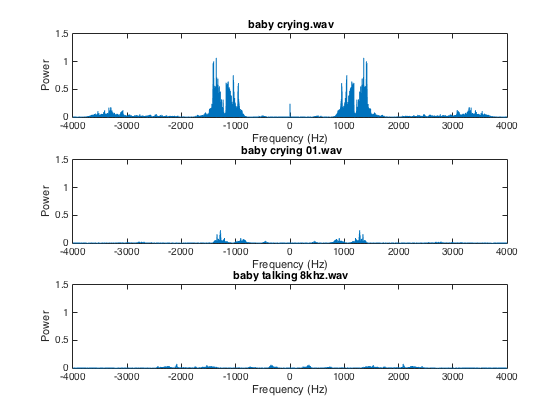
\includegraphics[width=1\textwidth]{sections/freq_spec_baby_linkaxis.png}
%  \caption{Frequency spectrum for baby sound files}
%  \label{fig:baby_spec}
%\end{figure}
%
%\begin{figure}[h]
%  \centering
%  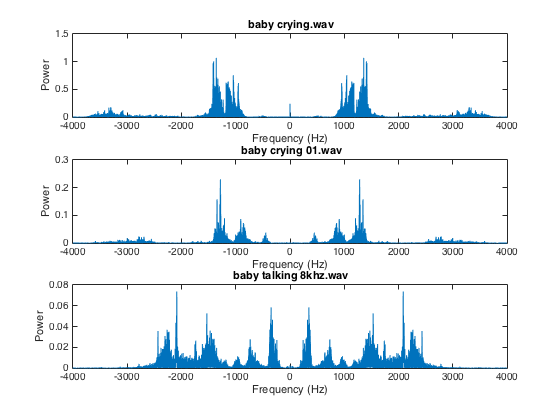
\includegraphics[width=1\textwidth]{sections/freq_spec_babyFix.png}
%  \caption{Frequency spectrum for baby sound files with scaled y-axis}
%  \label{fig:enhanced}
%\end{figure}

\begin{figure}[H]
  \centering
  \begin{minipage}[b]{0.6\textwidth}
    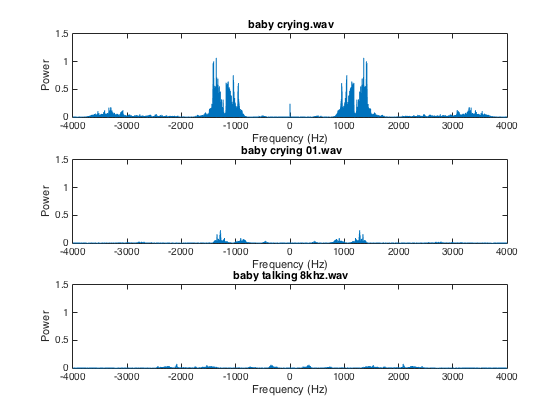
\includegraphics[width=1\textwidth]{sections/freq_spec_baby_linkaxis.png}
    \caption{Frequency spectrum for baby sound}
    \label{fig:baby_spec}
  \end{minipage}
  %\hfill
  \begin{minipage}[b]{0.6\textwidth}
    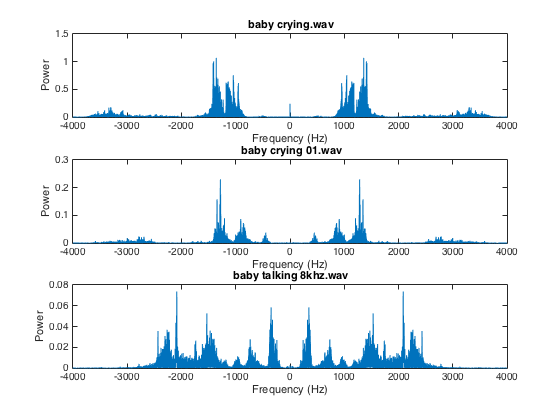
\includegraphics[width=1\textwidth]{sections/freq_spec_babyFix.png}
    \caption{Frequency spectrum for baby sound, scaled y-axis}
    \label{fig:enhanced}
  \end{minipage}
\end{figure}

\begin{figure}[H]
  \centering
  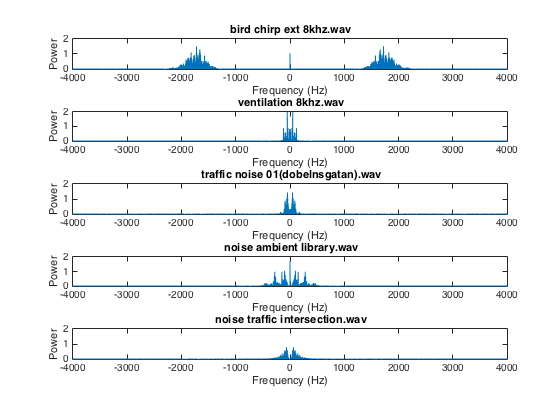
\includegraphics[width=1\textwidth]{sections/freq_spec_noise_2.png}
  \caption{Frequency spectrum for noise files}
  \label{fig:noise_spec}
\end{figure}

\subsection{The algorithms}
A quick and simple algorithm for a BAD application is preferably an algorithm that measures the 
energy from the input signal. Another benefit is that the implementation in Android OS may be easier
for a novice application developer.
Mathematically described, the power equation, which is close relationship to energy, is given by the following formula: 
\[
P(n) = \frac{1}{N} \sum\limits_{k=0}^{N-1} x^2(n-k)
\]
Since the BAD application will be performing energy calculations of the input signal in 
real-time, it is undoubtedly impossible to implement the equation. A solution to the problem is to use the 
\emph{recursive averaging} algorithm. It is a small and hardware friendly algorithm that calculates the energy 
levels of a given signal without using too much memory. Given the equation below,
\[
P(n) = \alpha P(n-1)+(1-\alpha)x^2(n)
\]
instead of performing the calculation for one sample at the time, a block of samples,referred to as frames,
are squared and summed. Each frame represents $x^2(n)$. The result, $P(n-1)$, is saved to be used as $P(n-1)$. 
The $\alpha$ is a constant between 0 and 1 and is related to the following formula:
\[
\alpha = \frac{1}{T_{s}F_{s}}
\]
Despite that the $\alpha$ can be derived from the equation, to get the better results further tweaking and testing is required.
The $\alpha$ value used in this research, $0.5$, suggests that the new $P(n)$ is equally weighted between old and new calculations.

The advanced algorithm is based upon the same, \emph{recursive averaging}, algorithm but before calculating
the average power the signal is first filtered through a Butterworth bandpass filter to remove unwanted 
frequencies. Butterworth because is gives the least amount of ripple in the bandpass. By having the noise frequencies suppressed, 
more precision is acquired for finding baby activity. The MATLAB code for the filter can be found in Appendix A.

\begin{figure}{H}
  \centering
  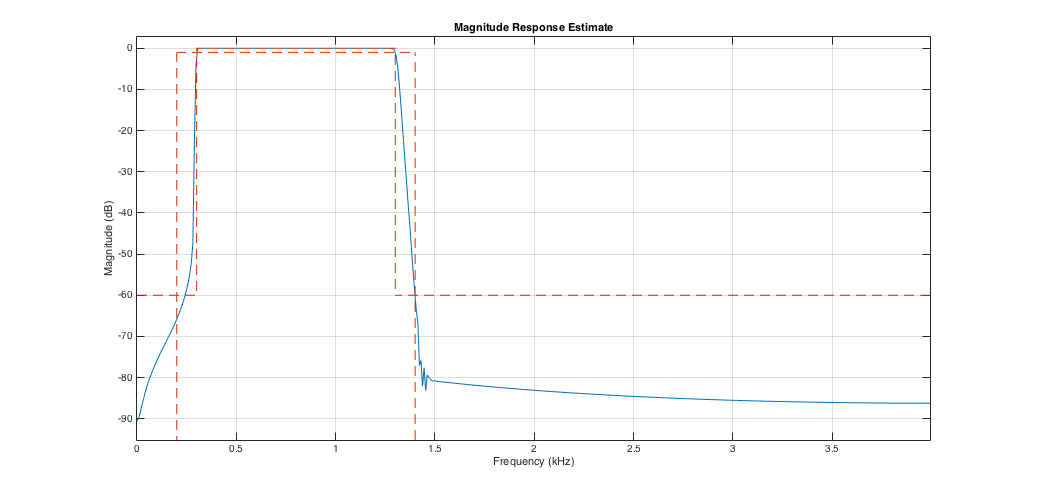
\includegraphics[width=1\textwidth]{sections/butt_pass_est.png}
  \caption{Butterworth 300-1300 Hz bandpass filter}
  \label{fig:butt_pass}
\end{figure}

\subsection{Evaluation and performance}
To evaluate and test the performance of the simple and advance algorithm new sound files were created. The three provided
baby sound files created the based. The goal was to make the alarm go off with the sound that the baby caused. 
For each baby sound file, three new sound files were created to mislead the algorithms.
The three tests configurations, with different baby base, contained the following files:

\begin{enumerate}
  \item clean, no without noise
  \item simulate early mornings, bird and ventilation noise added
  \item simulate noise environment, all noise files added
  \item simulate 'extreme' noise environment, all noise files added and amplified
\end{enumerate}

As can be seen from Figure \ref{fig:bc1_simp_crop}, the green horizontal line indicates the threshold value and the red horizontal line
suggest where a possible threshold could be placed. The red circle indicates when the alarm has been set off, when the algorithm has
notified that there is baby activity.

The results from \emph{Baby crying.wav}, Figure \ref{fig:bc1_simp}, test show that the alarm was set off in the same approximate time.
The reason for this could be that there is a high energy baby sound in the beginning of all of the files and hence why it triggered early.

\begin{figure}[H]
  \centering
  %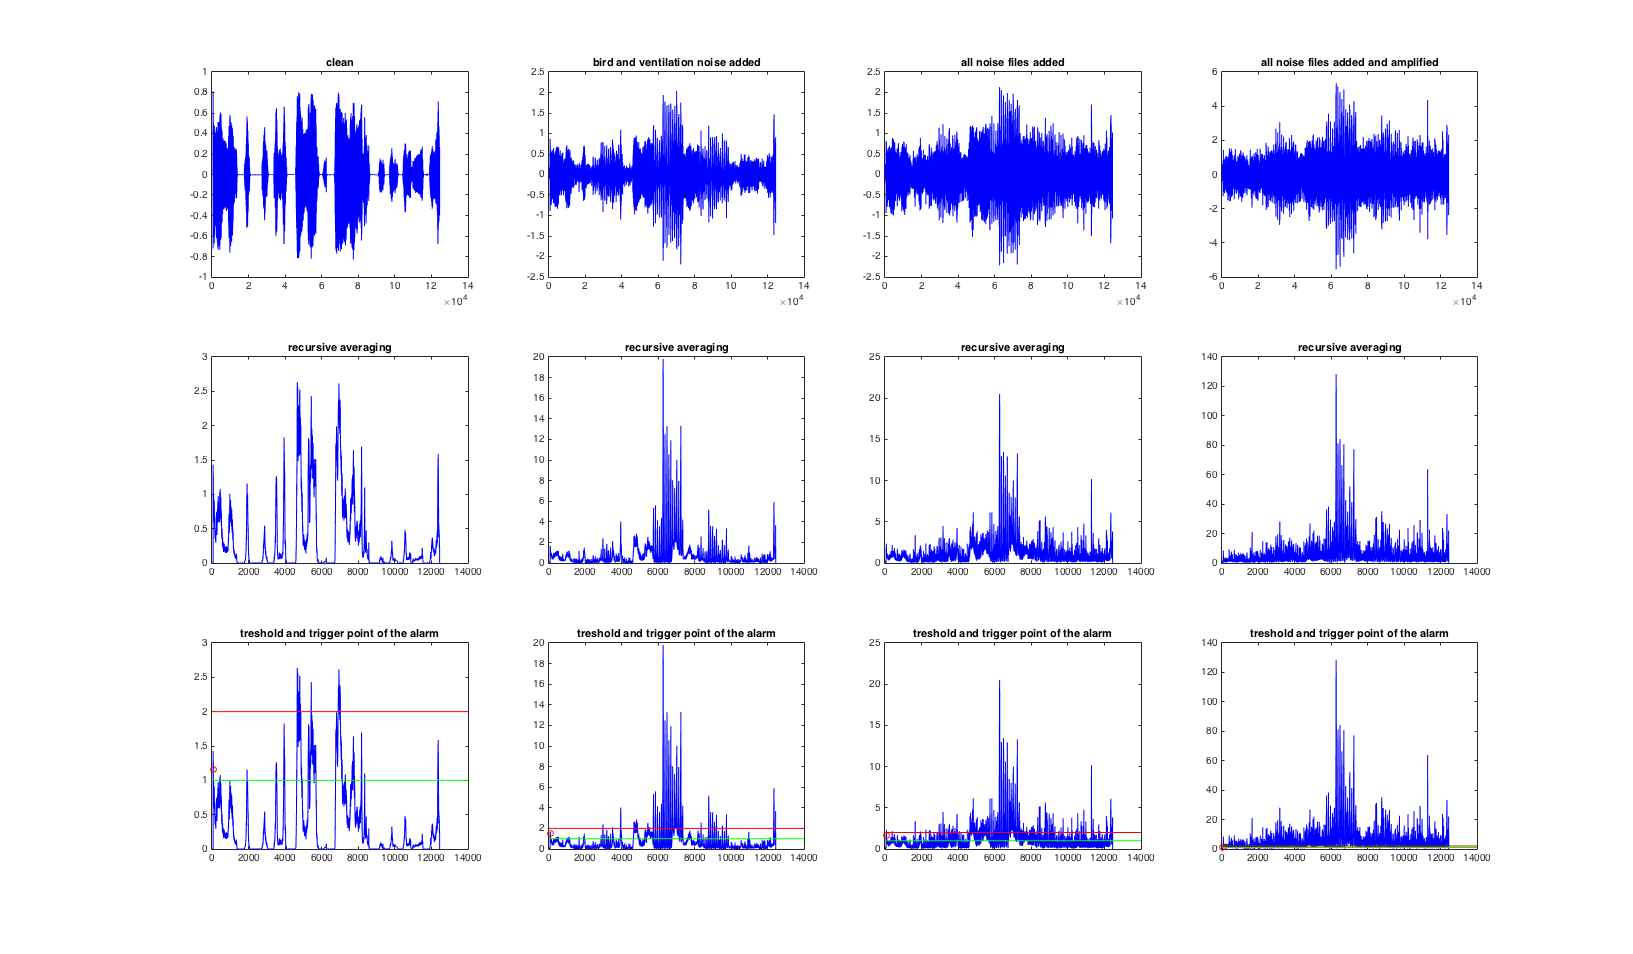
\includegraphics[width=1\textwidth]{sections/newFigures/bc1_unfilt.png}
  \makebox[\textwidth][c]{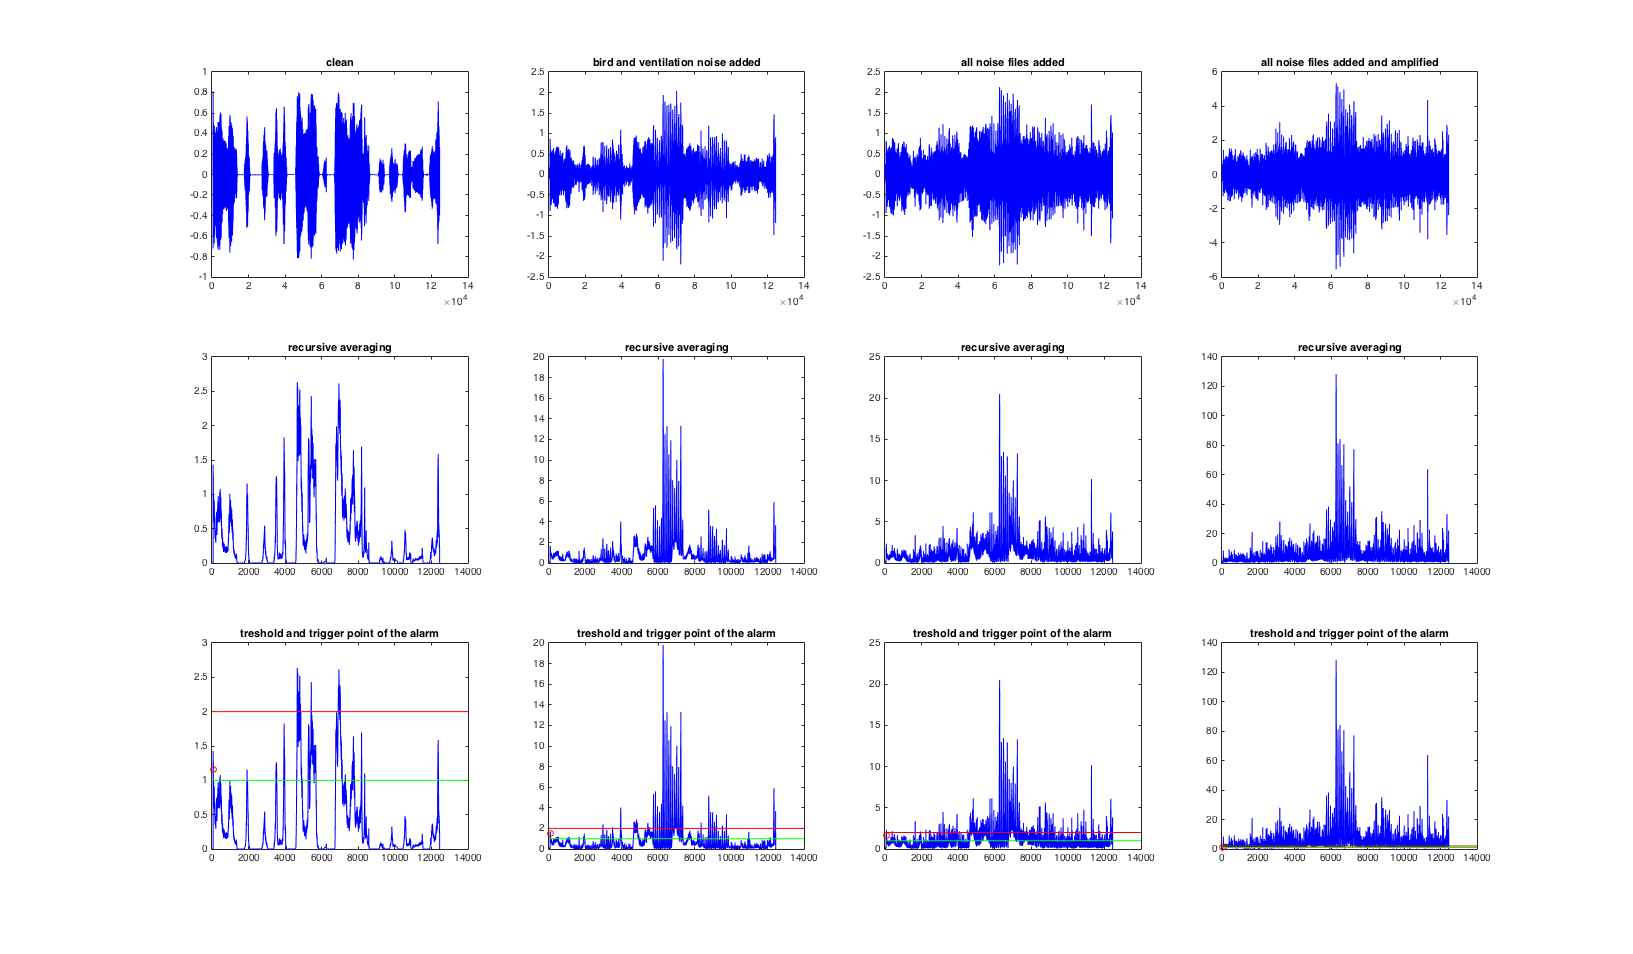
\includegraphics[width=1.5\textwidth]{sections/newFigures/bc1_unfilt.png}}
  \caption{Baby crying.wav, simple algorithm}
  \label{fig:bc1_simp}
\end{figure}

Figure \ref{fig:bc1_simp_crop} gives a doubt whether or not the noise could have set off the alarm.

\begin{figure}[H]
  \centering
  %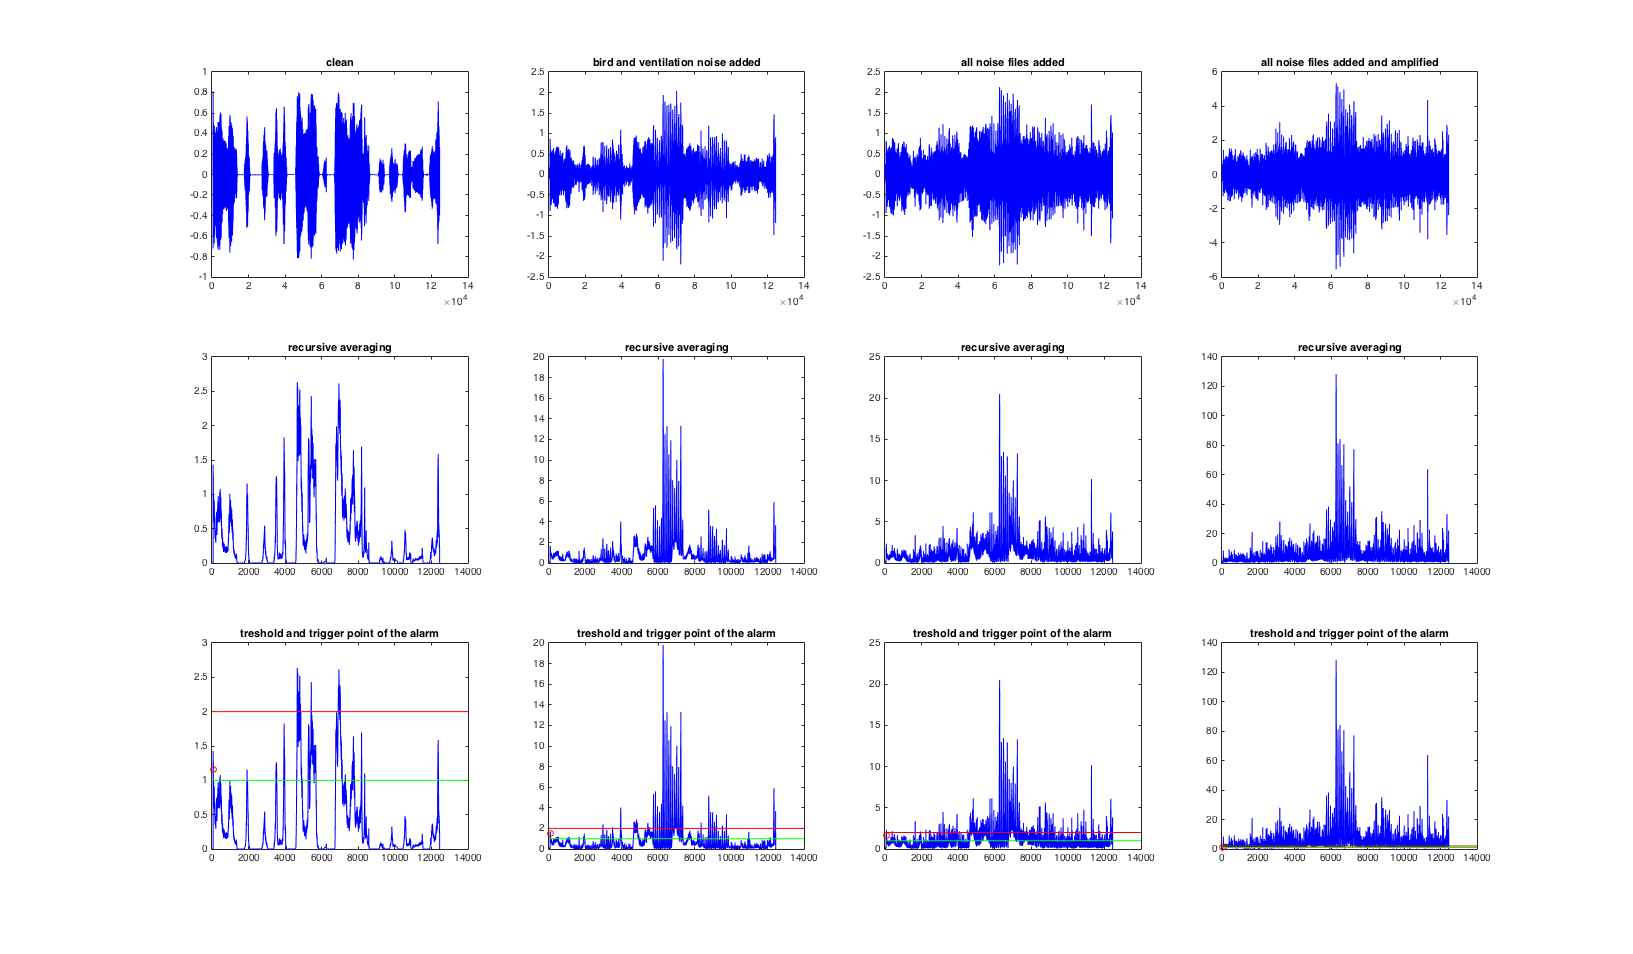
\includegraphics[width=1\textwidth]{sections/newFigures/bc1_unfilt.png}
  \makebox[\textwidth][c]{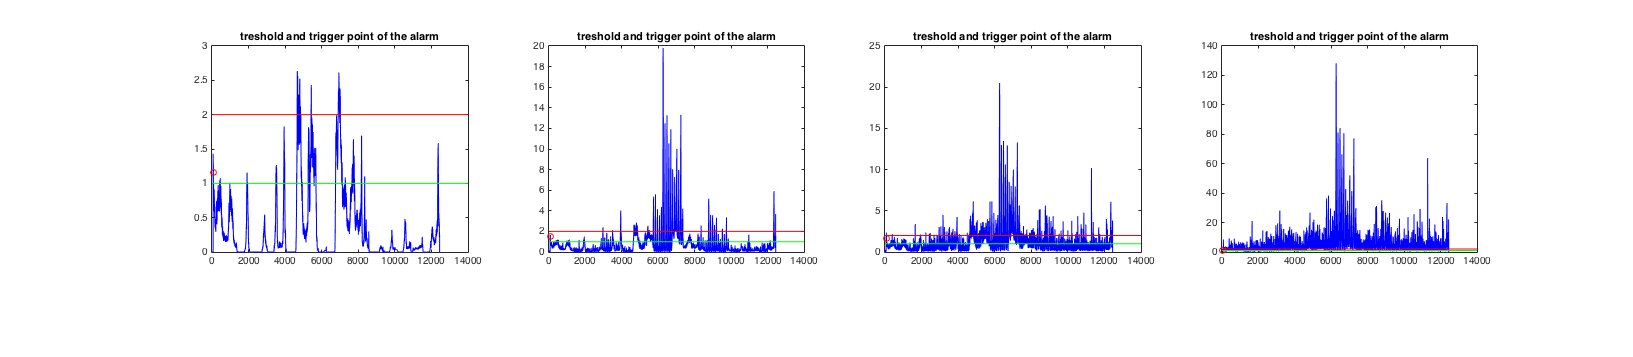
\includegraphics[width=1.5\textwidth]{sections/newFigures/bc1_unfilt_crop.png}}
  \caption{Baby crying.wav, simple algorithm}
  \label{fig:bc1_simp_crop}
\end{figure}

Both \emph{Baby crying1.wav} and \emph{Baby talking.wav} gave unsatisfactory results without any amplification, as 
can be seen in Figure \ref{fig:bc2_simp} and Figure \ref{fig:bt_simp}. Not remotely close to trigger the alarm in clean
configuration, illustrated be the left most plots, the test were performed a second time but with amplified baby sound.


\begin{figure}[H]
  \centering
  %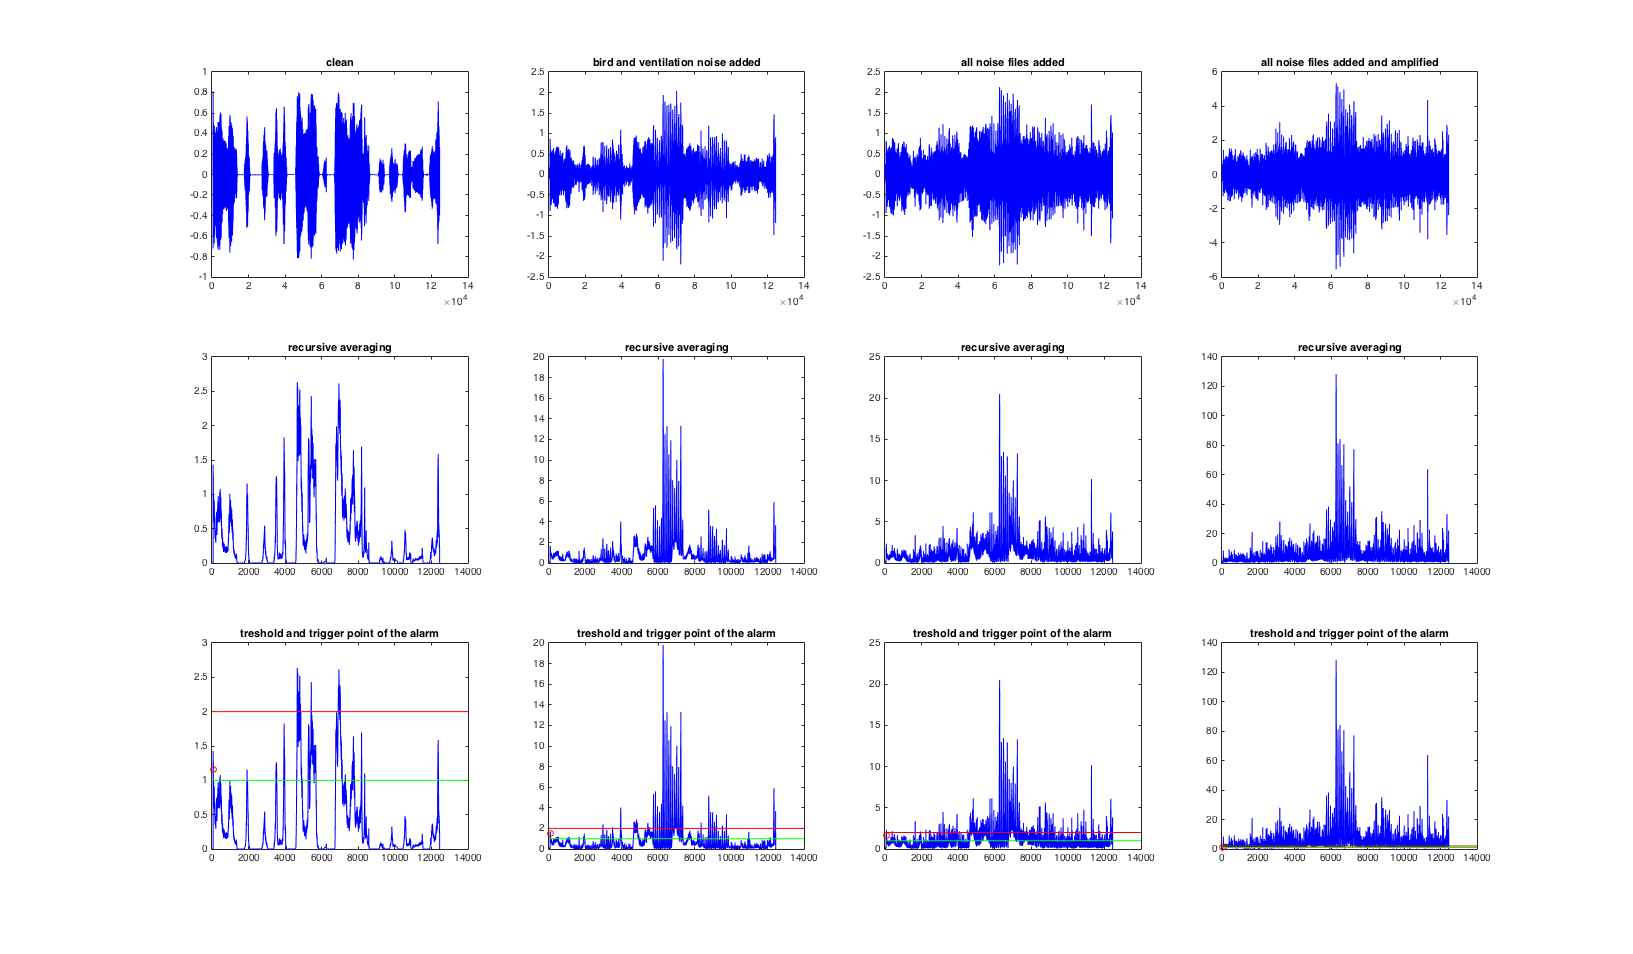
\includegraphics[width=1\textwidth]{sections/newFigures/bc1_unfilt.png}
  \makebox[\textwidth][c]{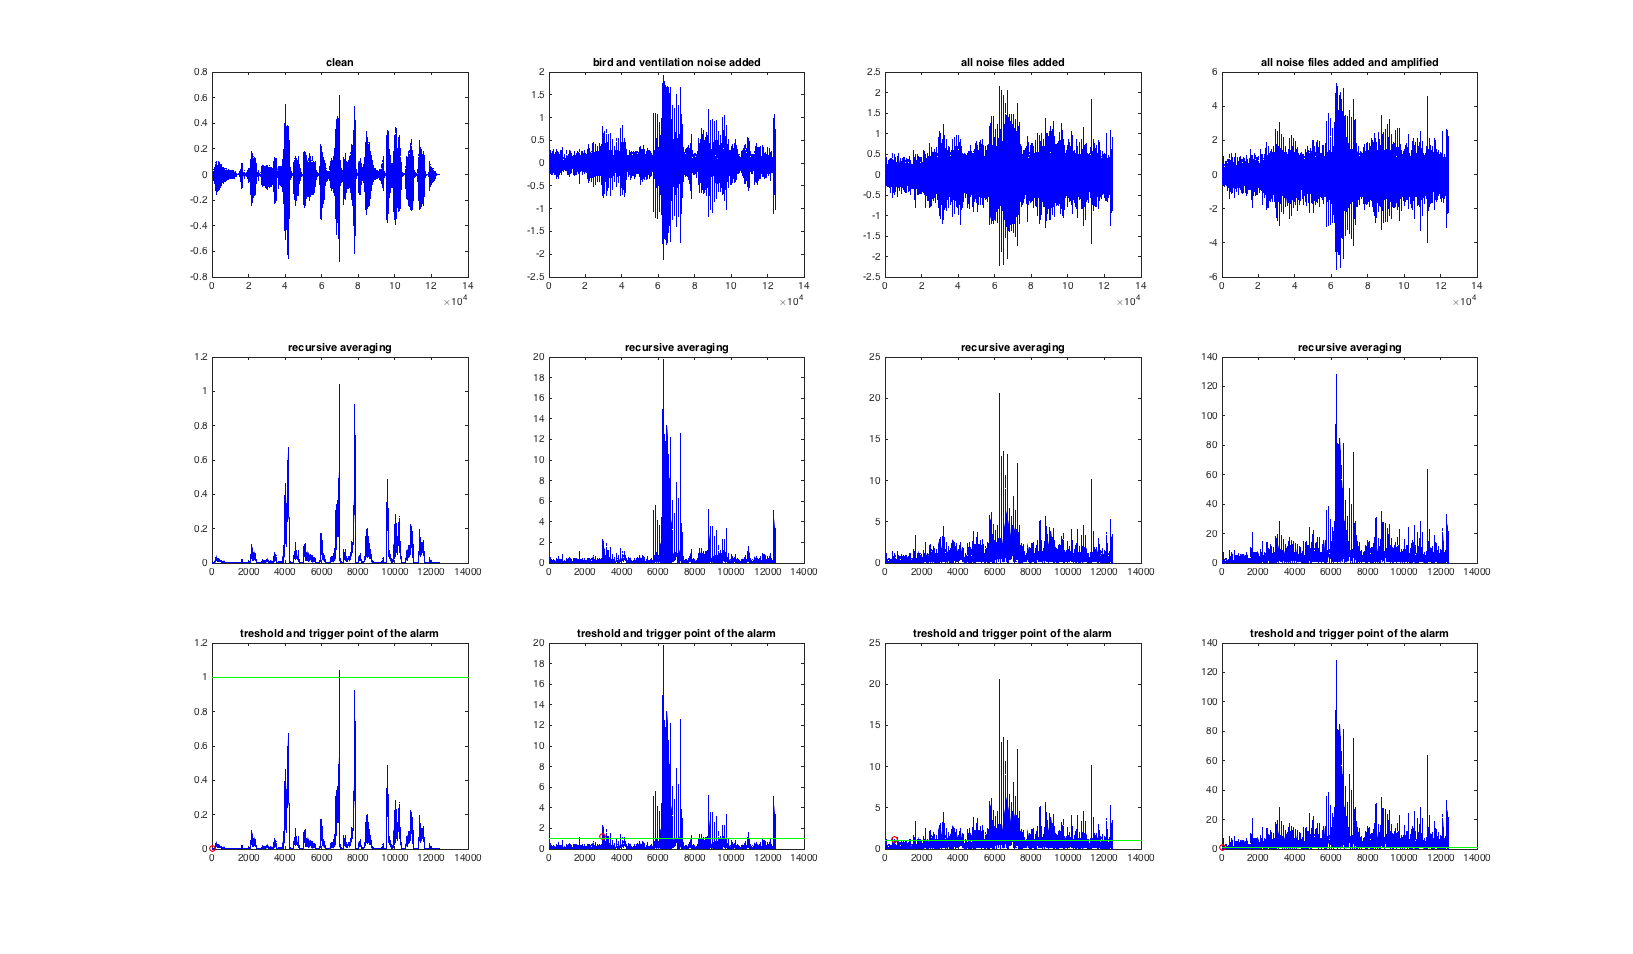
\includegraphics[width=1.5\textwidth]{sections/newFigures/bc2_unfilt.png}}
  \caption{Baby crying1.wav, simple algorithm}
  \label{fig:bc2_simp}
\end{figure}
\begin{figure}[H]
  \centering
  %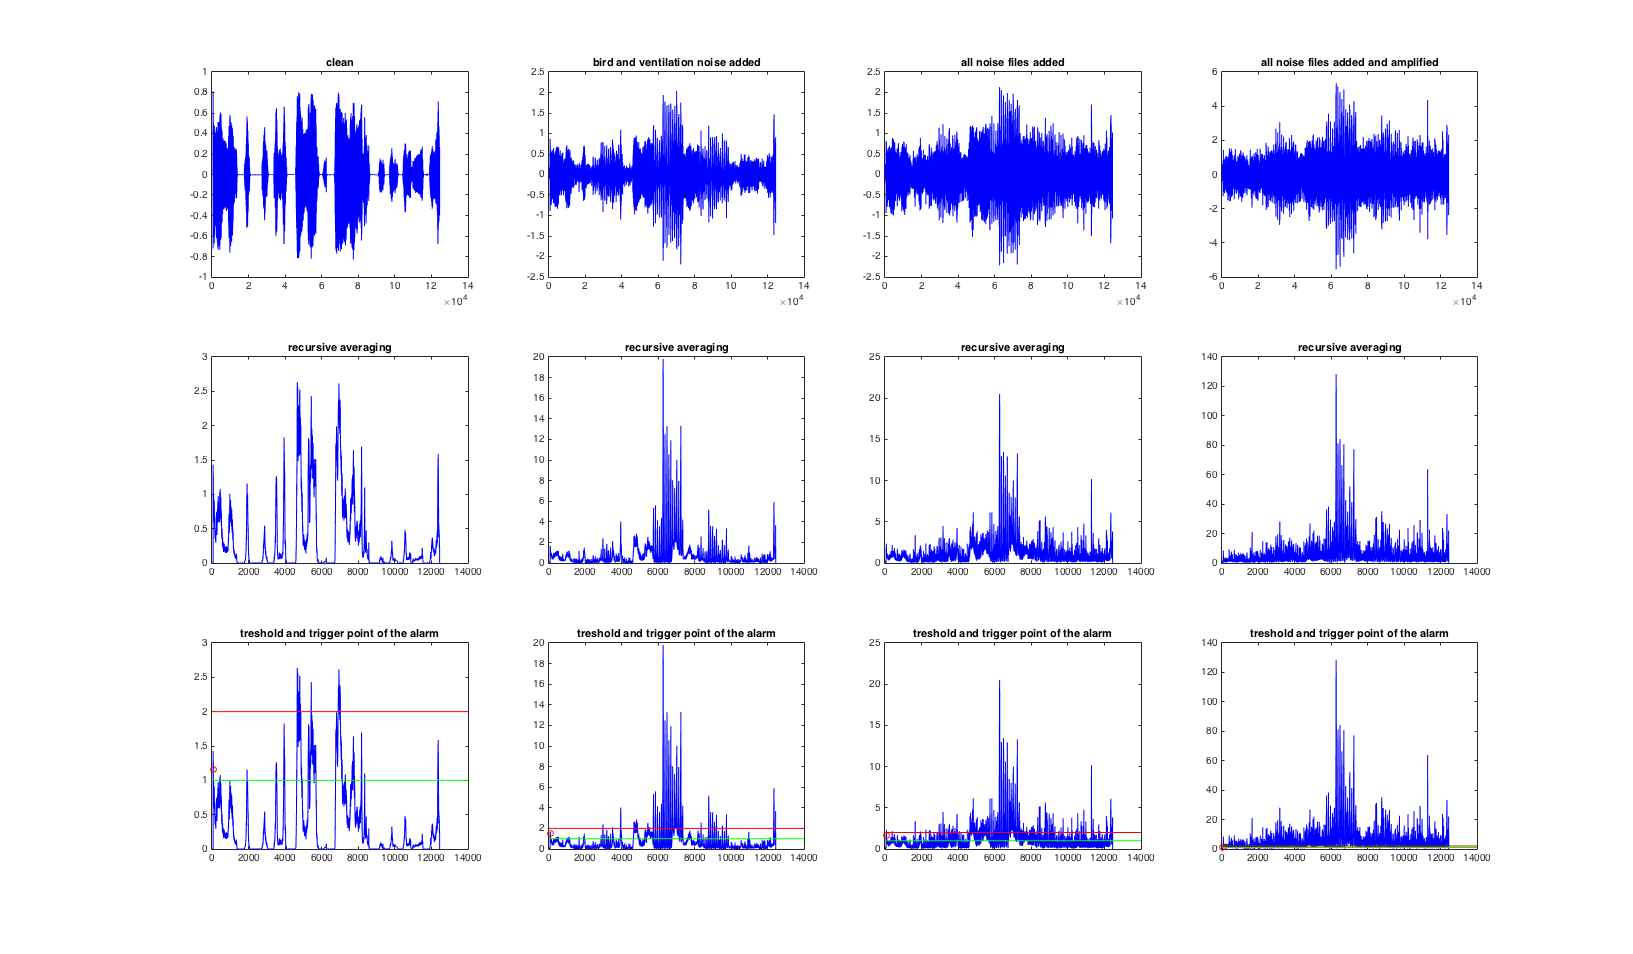
\includegraphics[width=1\textwidth]{sections/newFigures/bc1_unfilt.png}
  \makebox[\textwidth][c]{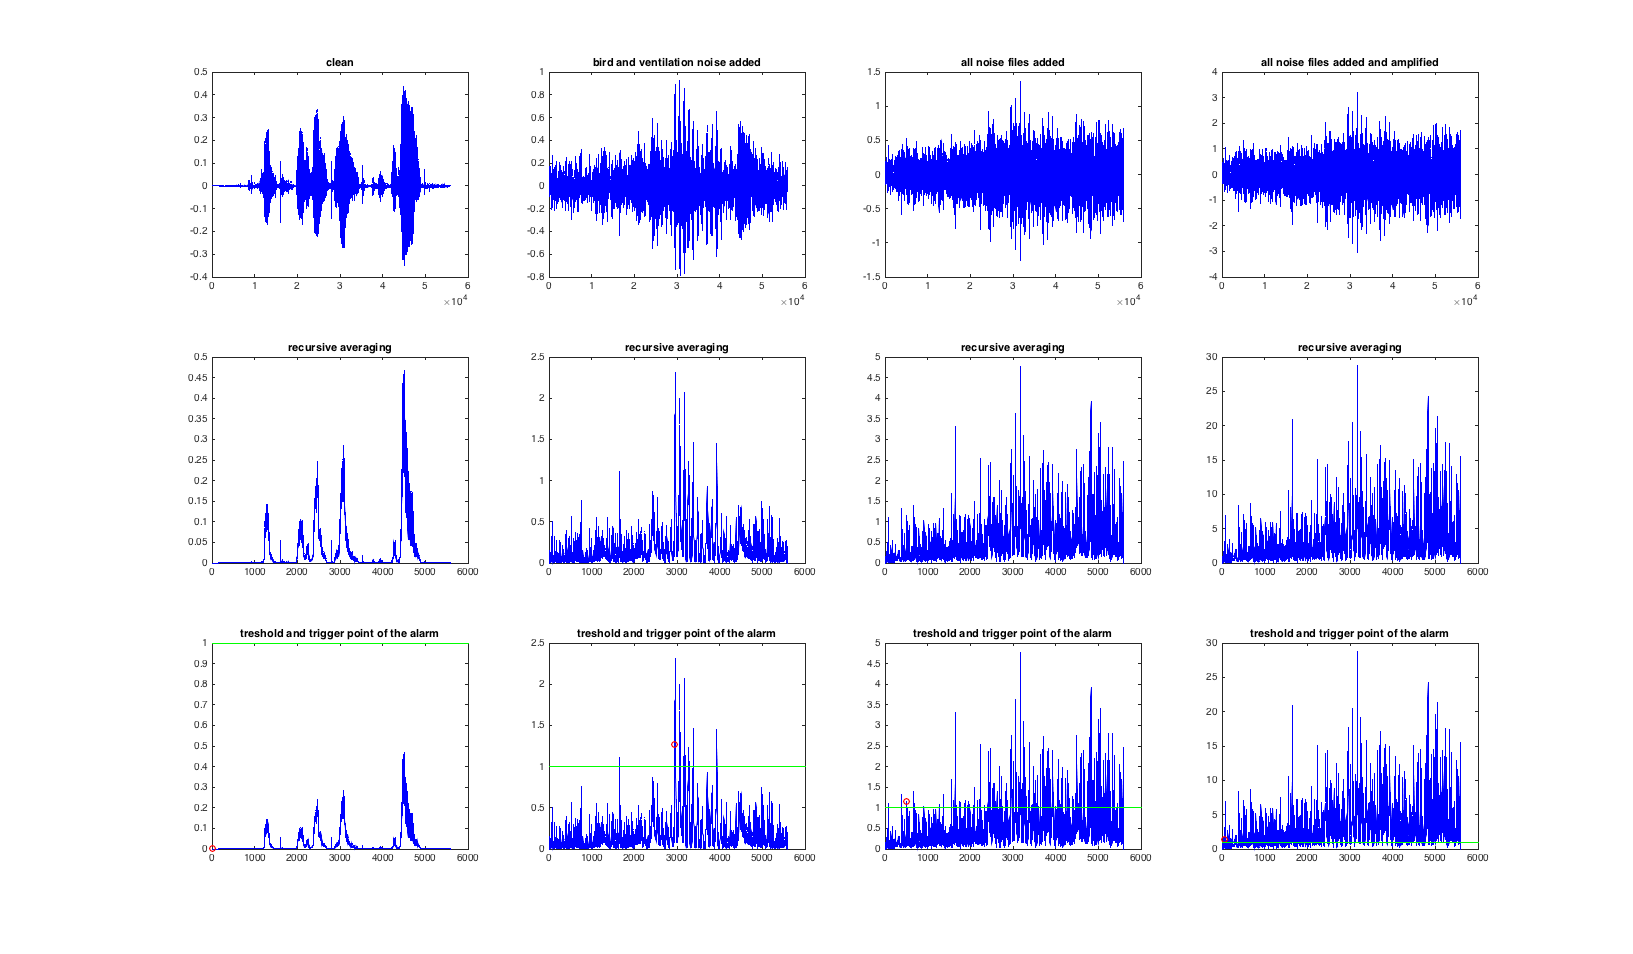
\includegraphics[width=1.5\textwidth]{sections/newFigures/bt_unfilt.png}}
  \caption{Baby talking.wav, simple algorithm}
  \label{fig:bt_simp}
\end{figure}

Figure \ref{fig:bc2_simp_amped} and Figure \ref{bt_simp_amped} 

\begin{figure}[H]
  \centering
  %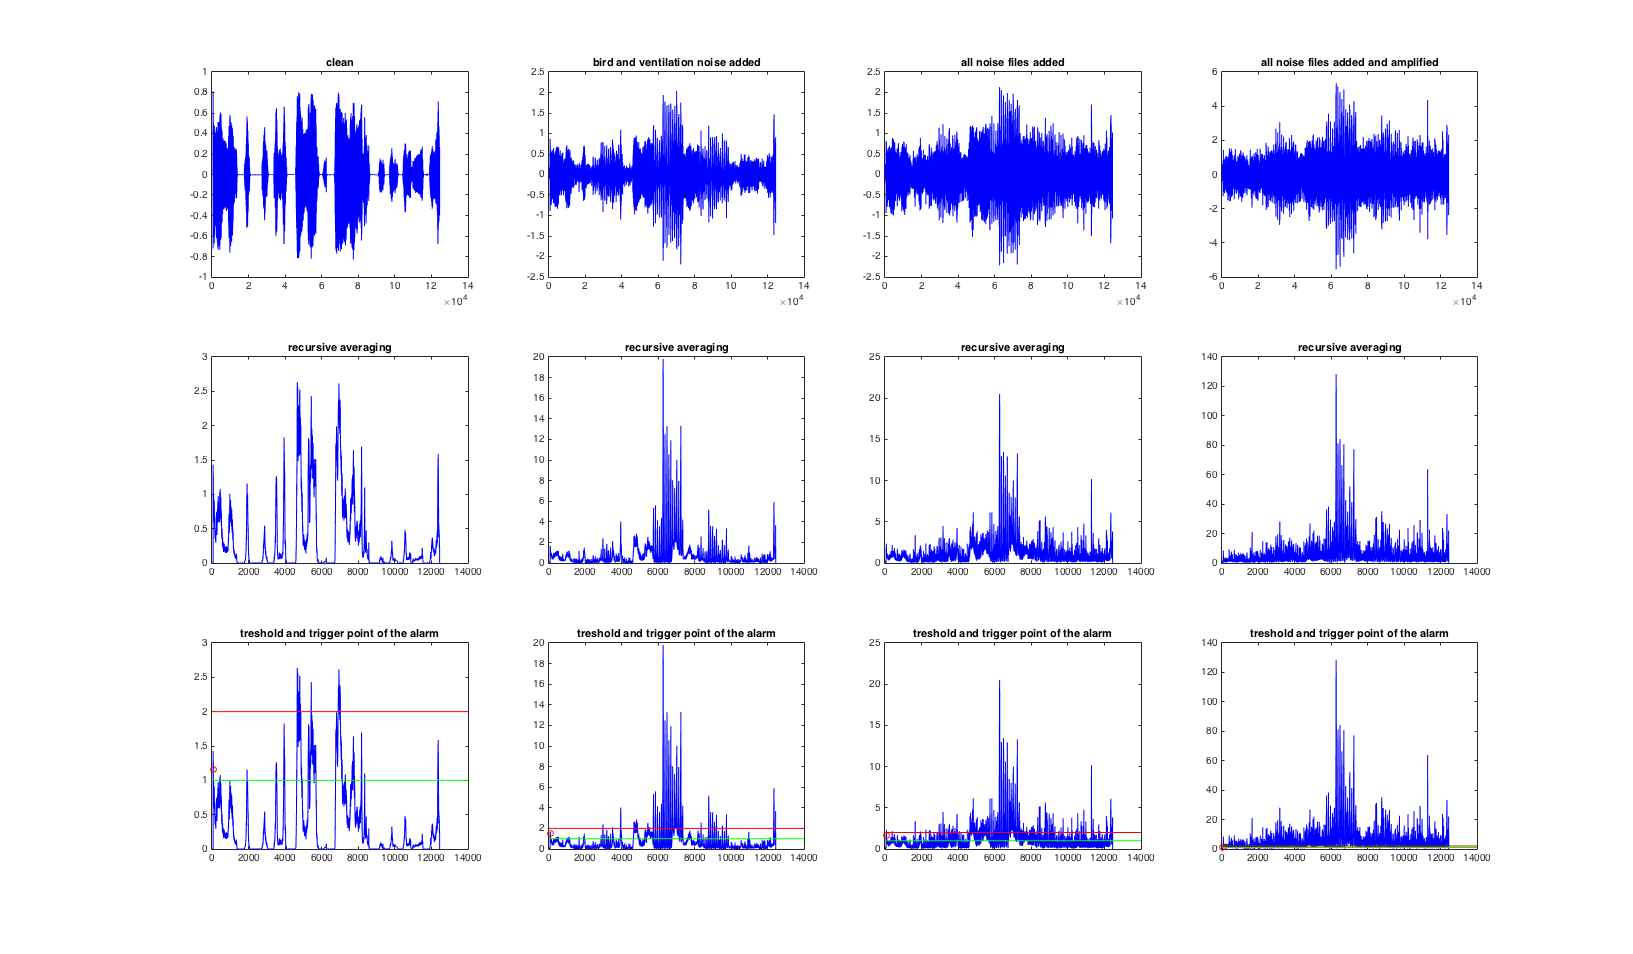
\includegraphics[width=1\textwidth]{sections/newFigures/bc1_unfilt.png}
  \makebox[\textwidth][c]{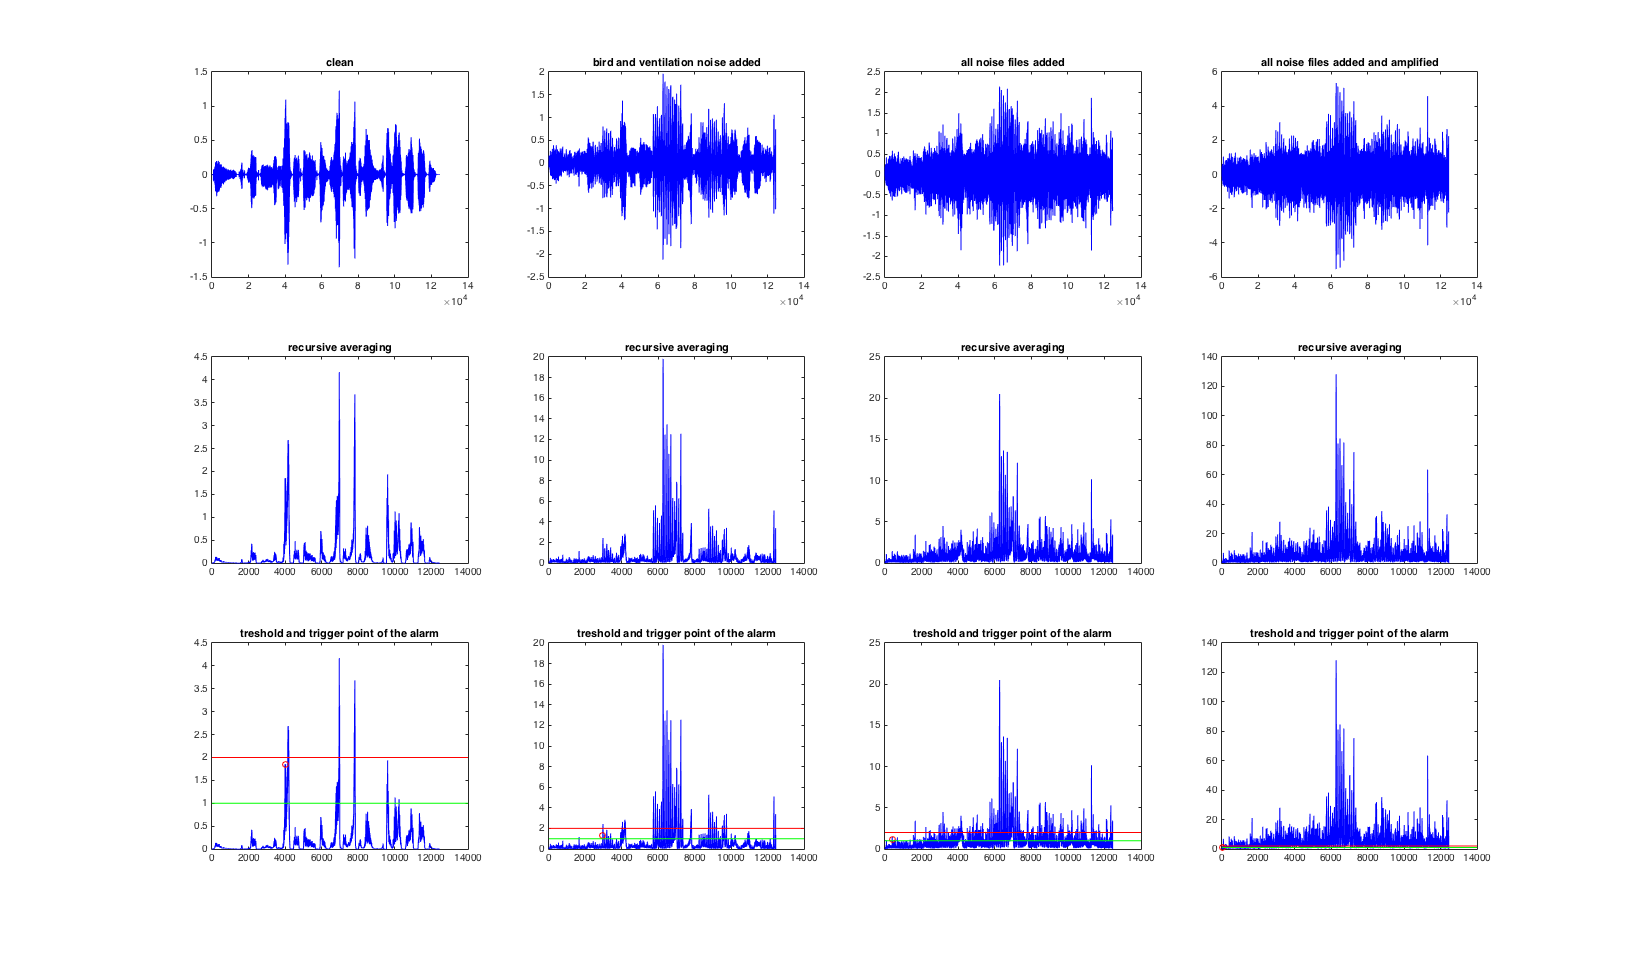
\includegraphics[width=1.5\textwidth]{sections/newFigures/bc2_unfilt_amped.png}}
  \caption{Amplified Baby crying1.wav, simple algorithm}
  \label{fig:bc2_simp_amped}
\end{figure}
\begin{figure}[H]
  \centering
  %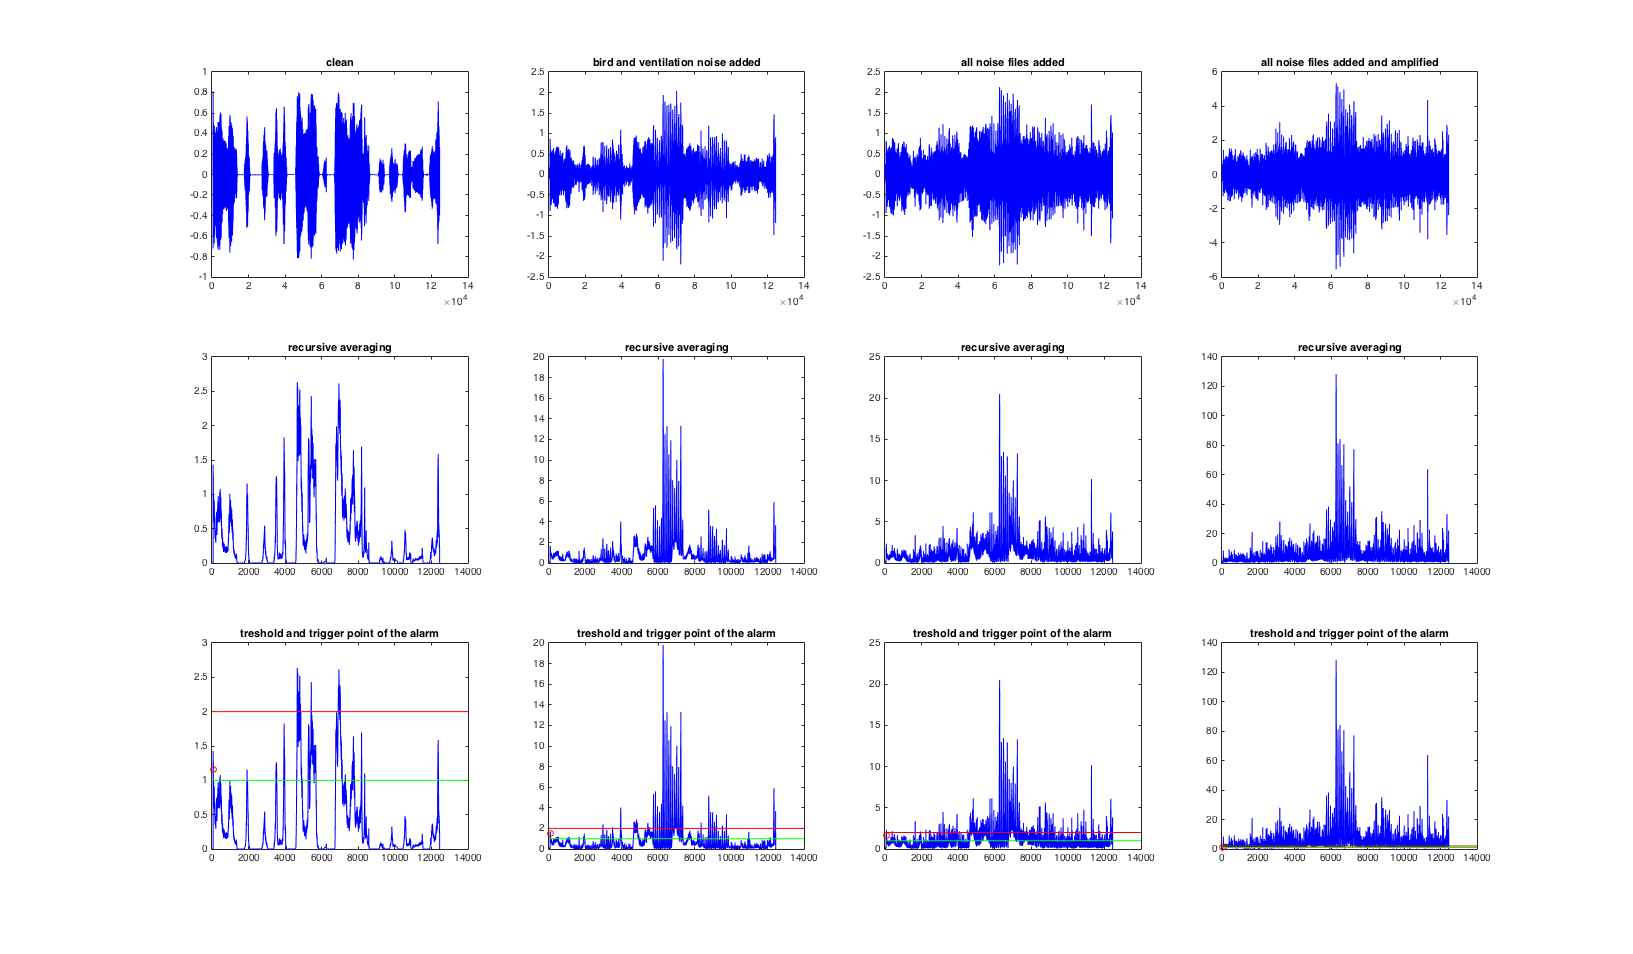
\includegraphics[width=1\textwidth]{sections/newFigures/bc1_unfilt.png}
  \makebox[\textwidth][c]{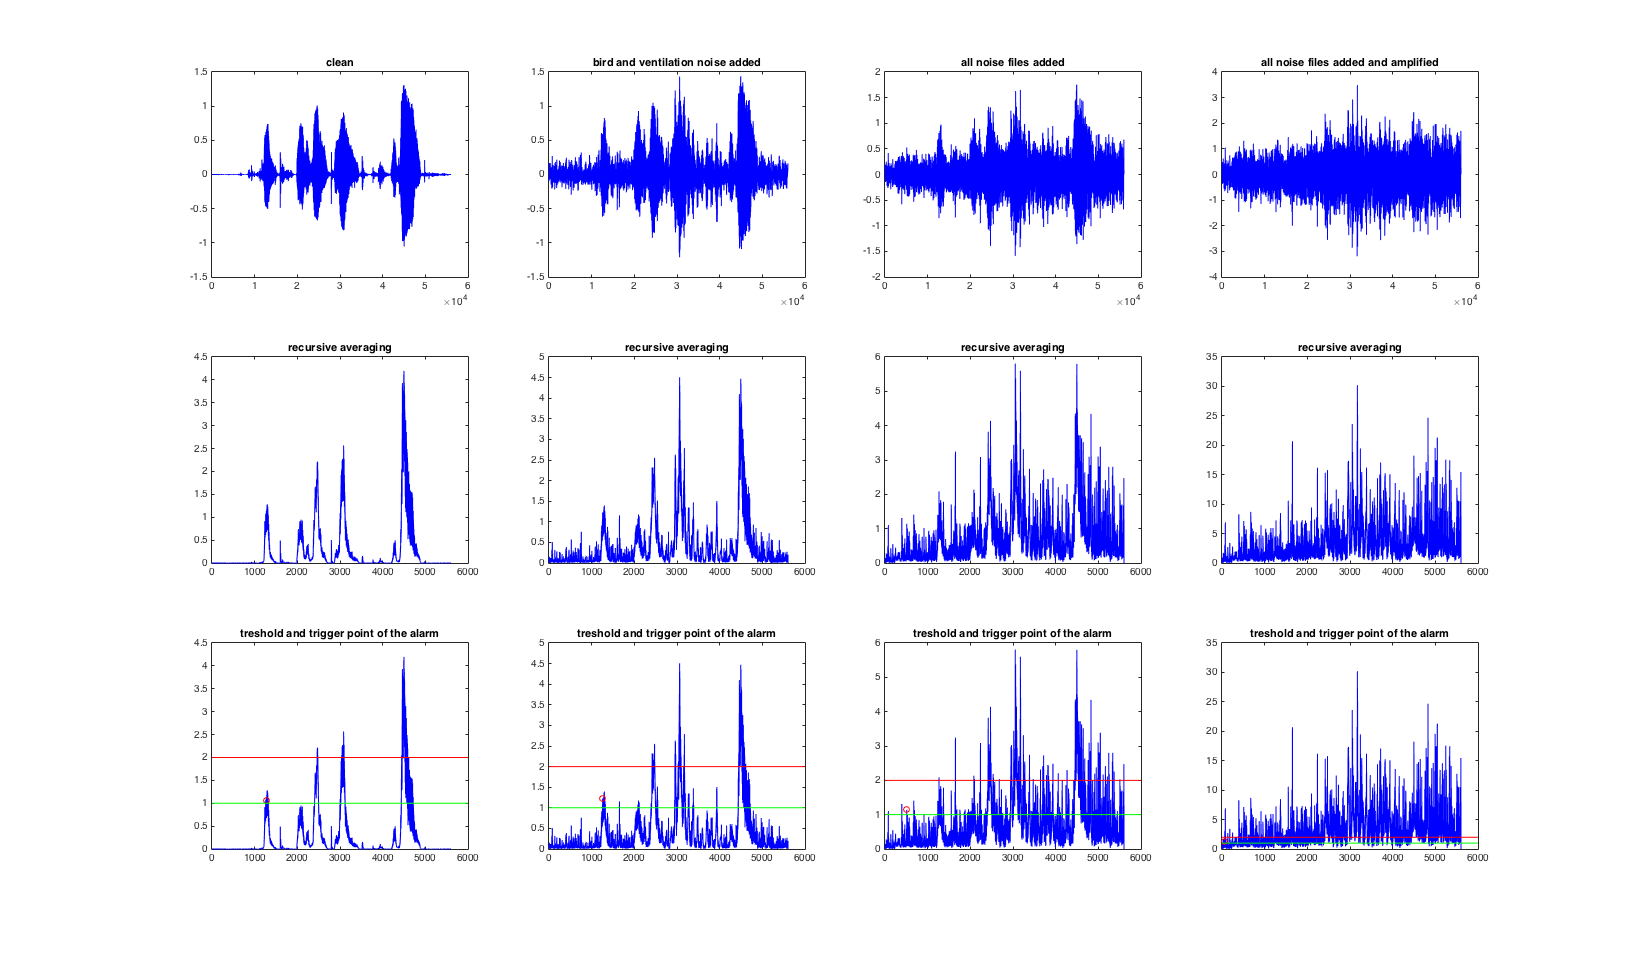
\includegraphics[width=1.5\textwidth]{sections/newFigures/bt_unfilt_amped.png}}
  \caption{Amplified Baby talking.wav, simple algorithm}
  \label{fig:bt_simp_amped}
\end{figure}
